% --- 付録 ---
\appendix
\section*{付録}

\begin{frame}{DCJ距離の下限}
    \begin{lemma}[DCJ距離の下限]
        任意の2つのゲノム $A, B$ について，DCJ距離は以下を満たす：
        \[
            d_{\mathrm{DCJ}}(A,B) \ge N - \left( C + \frac{I}{2} \right)
        \]
        ここで，$N$は遺伝子数，$C$は\textbf{隣接グラフ $AG(A,B)$ 上のサイクル}の個数，$I$は\textbf{隣接グラフ $AG(A,B)$ 上の奇数長パス}の個数である．
    \end{lemma}

    % ...existing code...
    \begin{alertblock}{成分の変化量に関する性質}
        \begin{itemize}
            \item DCJ操作によってサイクル数 $C$ と奇数長パス数 $I$ が\textbf{同時に増減することはない}．
            \item サイクル数 $C$ が増減するときは，最大で $1$ しか変わらない ($\Delta C \in \{0, \pm 1\}$)．
            \item 奇数長パス数 $I$ が変化するときは，$2, 0, -2$ しか変わらない ($\Delta I \in \{0, \pm 2\}$)．
        \end{itemize}
    \end{alertblock}
\end{frame}

% --- アルゴリズムの正当性 ---

\begin{frame}{アルゴリズムの正当性の根拠}
    \begin{block}{整数性}
        $C + I/2$ の変化量は常に $0$ または $\pm 1$ であり，DCJ操作ごとに距離 $d$ も整数として保たれる．
    \end{block}

    \begin{block}{最適性の保証}
        任意の $A \neq B$ に対し，必ず $d$ を $1$ 減少させるDCJ操作が存在する．
        したがって，距離公式の下限値は実際に達成可能である．
    \end{block}

    したがって，Lemma 3と以上の議論より，次の定理が導かれる．
\end{frame}

% 2. DCJ操作手順1
\begin{frame}{DCJ操作手順1}
    % ここに1手順目の図（例：初期状態）
    \begin{center}
    \scalebox{0.7}{
    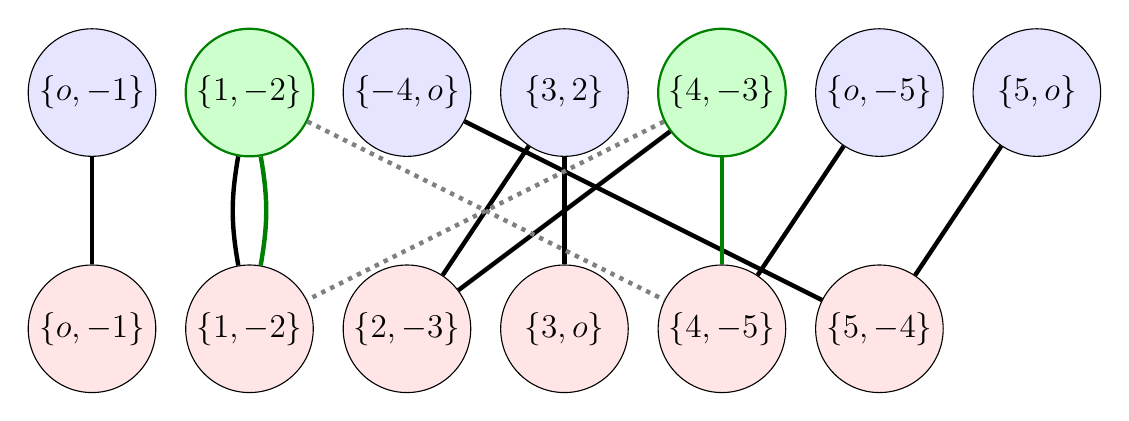
\begin{tikzpicture}[
        x = 2.0cm, y = 3.0cm,
        every node/.style={circle, draw, minimum size=1.62cm, inner sep=0pt, font=\large},
        adjA/.style={fill=blue!10},
        adjB/.style={fill=red!10},
        adjNew/.style={fill=green!20, draw=green!50!black, thick},
        edge/.style={-, ultra thick},
        edgeNew/.style={-, ultra thick, green!50!black}
    ]
        % Genome A nodes (top row)
        \node[adjA] (a1) at (0, 0) {$\{ o, -1 \}$};
        \node[adjNew] (a2) at (1, 0) {$\{ 1, -2 \}$};
        \node[adjA] (a3) at (2, 0) {$\{ -4, o \}$};
        \node[adjA] (a4) at (3, 0) {$\{ 3, 2 \}$};
        \node[adjNew] (a5) at (4, 0) {$\{ 4, -3 \}$};
        \node[adjA] (a6) at (5, 0) {$\{ o, -5 \}$};
        \node[adjA] (a7) at (6, 0) {$\{ 5, o \}$};

        % Genome B nodes (bottom row)
        \node[adjB] (b1) at (0, -1) {$\{ o, -1 \}$};
        \node[adjB] (b2) at (1, -1) {$\{ 1, -2 \}$};
        \node[adjB] (b3) at (2, -1) {$\{ 2, -3 \}$};
        \node[adjB] (b4) at (3, -1) {$\{ 3, o \}$};
        \node[adjB] (b5) at (4, -1) {$\{ 4, -5 \}$};
        \node[adjB] (b6) at (5, -1) {$\{ 5, -4 \}$};

        % Edges
        \draw[edge] (a1) -- (b1); % -1

        % Changed edges from a2 {1, -2}
        \draw[edge] (a2) to[bend right=10] (b2); % 1 in {1, -2}
        \draw[edgeNew] (a2) to[bend left=10] (b2);  % -2 in {1, -2}

        \draw[edge] (a3) -- (b6);

        \draw[edge] (a4) -- (b4); % 3
        \draw[edge] (a4) -- (b3); % 2

        % Changed edges from a5 {4, -3}
        \draw[edgeNew] (a5) -- (b5); % 4 in {4, -5}
        \draw[edge] (a5) -- (b3); % -3 in {2, -3}

        \draw[edge] (a6) -- (b5); % -5
        \draw[edge] (a7) -- (b6); % 5

        % --- Old connections (dotted) ---
        \draw[edge, dotted, gray] (a2) -- (b5);
        \draw[edge, dotted, gray] (a5) -- (b2);
    \end{tikzpicture}
    }
    \end{center}
    \small 2回目のDCJ操作適用後：$(1,4),\ (-2,-3)\ \rightarrow\ (1,-2),\ (4,-3)$
\end{frame}

% 3. DCJ操作手順2
\begin{frame}{DCJ操作手順2}

    % ここに2手順目の図（例：1回目のDCJ操作後）
    \begin{center}
    \scalebox{0.7}{
    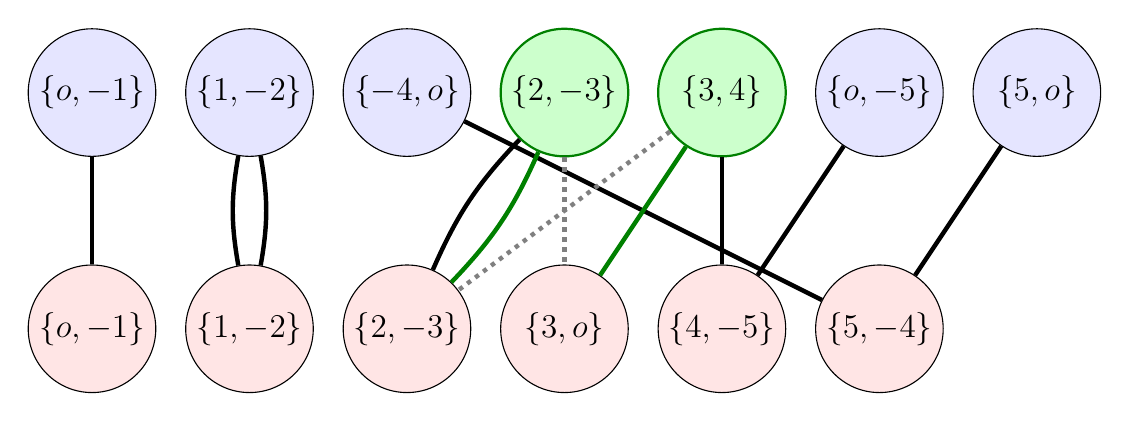
\begin{tikzpicture}[
        x = 2.0cm, y = 3.0cm,
        every node/.style={circle, draw, minimum size=1.62cm, inner sep=0pt, font=\large},
        adjA/.style={fill=blue!10},
        adjB/.style={fill=red!10},
        adjNew/.style={fill=green!20, draw=green!50!black, thick},
        edge/.style={-, ultra thick},
        edgeNew/.style={-, ultra thick, green!50!black}
    ]
        % Genome A nodes (top row)
        \node[adjA] (a1) at (0, 0) {$\{ o, -1 \}$};
        \node[adjA] (a2) at (1, 0) {$\{ 1, -2 \}$};
        \node[adjA] (a3) at (2, 0) {$\{ -4, o \}$};
        \node[adjNew] (a4) at (3, 0) {$\{ 2, -3 \}$};
        \node[adjNew] (a5) at (4, 0) {$\{ 3, 4 \}$};
        \node[adjA] (a6) at (5, 0) {$\{ o, -5 \}$};
        \node[adjA] (a7) at (6, 0) {$\{ 5, o \}$};

        % Genome B nodes (bottom row)
        \node[adjB] (b1) at (0, -1) {$\{ o, -1 \}$};
        \node[adjB] (b2) at (1, -1) {$\{ 1, -2 \}$};
        \node[adjB] (b3) at (2, -1) {$\{ 2, -3 \}$};
        \node[adjB] (b4) at (3, -1) {$\{ 3, o \}$};
        \node[adjB] (b5) at (4, -1) {$\{ 4, -5 \}$};
        \node[adjB] (b6) at (5, -1) {$\{ 5, -4 \}$};

        % Edges
        \draw[edge] (a1) -- (b1); % -1
        \draw[edge] (a2) to[bend right=10] (b2); % 1 in {1, -2}
        \draw[edge] (a2) to[bend left=10] (b2);  % -2 in {1, -2}
        \draw[edge] (a3) -- (b6); % -4
        \draw[edge] (a4) to[bend right=10] (b3); % 2,-3 (1本目, 緑)
        \draw[edgeNew] (a4) to[bend left=10] (b3);  % 2,-3 (2本目, 緑)
        \draw[edgeNew] (a5) -- (b4); % 3,4
        \draw[edge] (a5) -- (b5); % 4 in {4, -5}
        \draw[edge] (a6) -- (b5); % -5
        \draw[edge] (a7) -- (b6); % 5

        % --- Old connections (dotted) ---
        \draw[edge, dotted, gray] (a4) -- (b4);
        \draw[edge, dotted, gray] (a5) -- (b3);
    \end{tikzpicture}
    }
    \end{center}
    \small 2回目のDCJ操作適用後：$(2,3),\ (-3,4)\ \rightarrow\ (2,-3),\ (3,o)$
\end{frame}

% 4. DCJ操作手順3
\begin{frame}{DCJ操作手順3}
    % 3回目のDCJ操作後の図
    \begin{center}
    \scalebox{0.7}{
    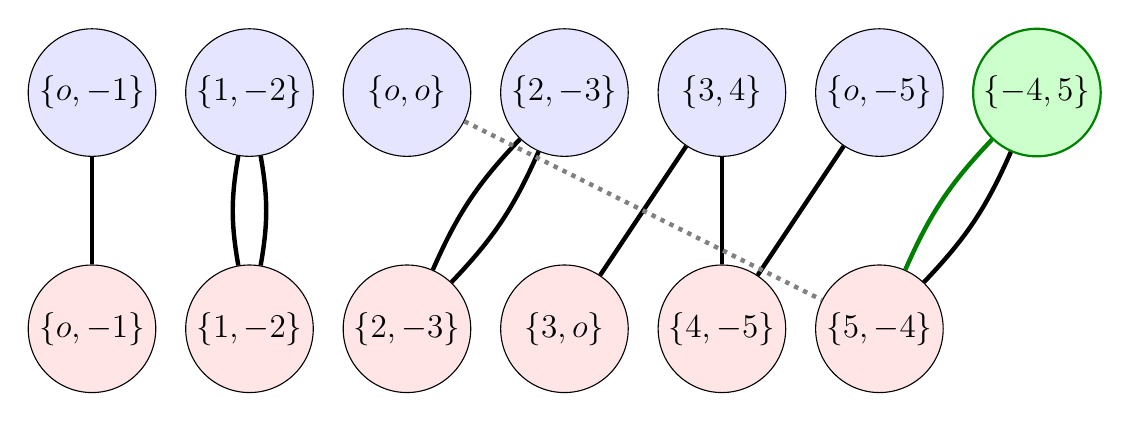
\begin{tikzpicture}[
        x = 2.0cm, y = 3.0cm,
        every node/.style={circle, draw, minimum size=1.62cm, inner sep=0pt, font=\large},
        adjA/.style={fill=blue!10},
        adjB/.style={fill=red!10},
        adjNew/.style={fill=green!20, draw=green!50!black, thick},
        edge/.style={-, ultra thick},
        edgeNew/.style={-, ultra thick, green!50!black}
    ]
        % Genome A nodes (top row)
        \node[adjA] (a1) at (0, 0) {$\{ o, -1 \}$};
        \node[adjA] (a2) at (1, 0) {$\{ 1, -2 \}$};
        \node[adjA] (a3) at (2, 0) {$\{ o, o \}$};
        \node[adjA] (a4) at (3, 0) {$\{ 2, -3 \}$};
        \node[adjA] (a5) at (4, 0) {$\{ 3, 4 \}$};
        \node[adjA] (a6) at (5, 0) {$\{ o, -5 \}$};
        \node[adjNew] (a7) at (6, 0) {$\{ -4, 5 \}$};

        % Genome B nodes (bottom row)
        \node[adjB] (b1) at (0, -1) {$\{ o, -1 \}$};
        \node[adjB] (b2) at (1, -1) {$\{ 1, -2 \}$};
        \node[adjB] (b3) at (2, -1) {$\{ 2, -3 \}$};
        \node[adjB] (b4) at (3, -1) {$\{ 3, o \}$};
        \node[adjB] (b5) at (4, -1) {$\{ 4, -5 \}$};
        \node[adjB] (b6) at (5, -1) {$\{ 5, -4 \}$};

        % Edges
        \draw[edge] (a1) -- (b1); % -1
        \draw[edge] (a2) to[bend right=10] (b2); % 1 in {1, -2}
        \draw[edge] (a2) to[bend left=10] (b2);  % -2 in {1, -2}
        \draw[edge] (a4) to[bend right=10] (b3); % 2,-3 (1本目, 緑)
        \draw[edge] (a4) to[bend left=10] (b3);  % 2,-3 (2本目, 緑)
        \draw[edge] (a5) -- (b4); % 3,4
        \draw[edge] (a5) -- (b5); % 4 in {4, -5}
        \draw[edge] (a6) -- (b5); % -5
				\draw[edgeNew] (a7) to[bend right=10] (b6); % 2,-3 (1本目, 緑)
				\draw[edge] (a7) to[bend left=10] (b6);  % 2,-3 (2本目, 緑)

        % --- Old connections (dotted) ---
        \draw[edge, dotted, gray] (a3) -- (b6);
			\end{tikzpicture}
    }
    \end{center}
    \small 3回目のDCJ操作適用後：$(-4,o),\ (5,o)\ \rightarrow\ (-4,5),\ (o,o)$
\end{frame}

% 4. DCJ操作手順4
\begin{frame}{DCJ操作手順4}
    % 3回目のDCJ操作後の図
    \begin{center}
    \scalebox{0.7}{
    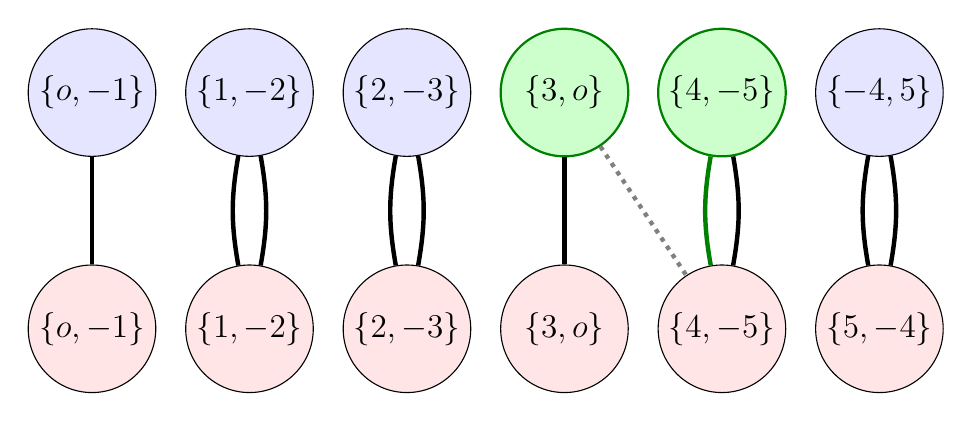
\begin{tikzpicture}[
        x = 2.0cm, y = 3.0cm,
        every node/.style={circle, draw, minimum size=1.62cm, inner sep=0pt, font=\large},
        adjA/.style={fill=blue!10},
        adjB/.style={fill=red!10},
        adjNew/.style={fill=green!20, draw=green!50!black, thick},
        edge/.style={-, ultra thick},
        edgeNew/.style={-, ultra thick, green!50!black}
    ]
        % Genome A nodes (top row)
        \node[adjA] (a1) at (0, 0) {$\{ o, -1 \}$};
        \node[adjA] (a2) at (1, 0) {$\{ 1, -2 \}$};
        % \node[adjA] (a3) at (2, 0) {$\{ o, o \}$};
        \node[adjA] (a4) at (2, 0) {$\{ 2, -3 \}$};
        \node[adjNew] (a5) at (3, 0) {$\{ 3, o \}$};
        \node[adjNew] (a6) at (4, 0) {$\{ 4, -5 \}$};
        \node[adjA] (a7) at (5, 0) {$\{ -4, 5 \}$};

        % Genome B nodes (bottom row)
        \node[adjB] (b1) at (0, -1) {$\{ o, -1 \}$};
        \node[adjB] (b2) at (1, -1) {$\{ 1, -2 \}$};
        \node[adjB] (b3) at (2, -1) {$\{ 2, -3 \}$};
        \node[adjB] (b4) at (3, -1) {$\{ 3, o \}$};
        \node[adjB] (b5) at (4, -1) {$\{ 4, -5 \}$};
        \node[adjB] (b6) at (5, -1) {$\{ 5, -4 \}$};

        % Edges
        \draw[edge] (a1) -- (b1); % -1
        \draw[edge] (a2) to[bend right=10] (b2); % 1 in {1, -2}
        \draw[edge] (a2) to[bend left=10] (b2);  % -2 in {1, -2}
        \draw[edge] (a4) to[bend right=10] (b3); % 2,-3 (1本目, 緑)
        \draw[edge] (a4) to[bend left=10] (b3);  % 2,-3 (2本目, 緑)
        \draw[edge] (a5) -- (b4); % 3,4
        % \draw[edge] (a5) -- (b5); % 4 in {4, -5}
				\draw[edgeNew] (a6) to[bend right=10] (b5); % 2,-3 (1本目, 緑)
				\draw[edge] (a6) to[bend left=10] (b5);  % 2,-3 (2本目, 緑)
				\draw[edge] (a7) to[bend right=10] (b6); % 2,-3 (1本目, 緑)
				\draw[edge] (a7) to[bend left=10] (b6);  % 2,-3 (2本目, 緑)

        % --- Old connections (dotted) ---
        \draw[edge, dotted, gray] (a5) -- (b5);
			\end{tikzpicture}
    }
    \end{center}
    \small 4回目のDCJ操作適用後：$(4,3),\ (-5,o)\ \rightarrow\ (4,-5),\ (3,o)$
\end{frame}

\begin{frame}{benchmark-読み込み含む}

	\begin{table}[H]
			\centering
			\caption{全体実行時間（読み込み・構築含む）とメモリ使用量}
			\label{tab:benchmark_total}
			\begin{tabular}{rcc}
					\hline
					遺伝子数 ($N$) & 実行時間 (sec) & メモリ使用量 (MB) \\
					\hline
					10      & 0.001 & 0.003 \\
					100     & 0.001 & 0.03 \\
					1,000   & 0.007 & 0.26 \\
					10,000  & 0.179 & 2.55 \\
					100,000 & 20.827 & 25.55 \\
					\hline
			\end{tabular}
	\end{table}
\end{frame}

\begin{frame}{benchmark-読み込み除く}
	\begin{table}[H]
			\centering
			\caption{アルゴリズム実行時間（読み込み・構築除く）}
			\label{tab:benchmark_algo}
			\begin{tabular}{rc}
					\hline
					遺伝子数 ($N$) & 実行時間 (sec) \\
					\hline
					10      & 0.001 \\
					100     & 0.001 \\
					1,000   & 0.002 \\
					10,000  & 0.005 \\
					100,000 & 0.051 \\
					\hline
			\end{tabular}
	\end{table}
\end{frame}
